\section{Конструкторская часть}
\subsection{IDEF0 диаграмма}
На рисунках \ref{idef0:top} -- \ref{idef0:A3} представленна IDEF0 диаграмма.

\begin{figure}[h]
	\begin{center}
		{\includegraphics[scale=0.63, angle=-90, page=1]{img/idef0/idef0.pdf}}
		\caption{IDEF0, контекстная диаграмма А0}
		\label{idef0:top}
	\end{center}
\end{figure}

Метод состоит из нескольких этапов, описанных на рисунке \ref{idef0:A0}. В первую строится опорный план грузоперевозок по модифицированному методу минимального элемента. Далее для него применяется также изменённый под условия решаемой задачи метод потенциалов. Результатом конечного числа итераций данного метода становится оптимальный набор маршрутов перевозки. По нему составляется расписание с использованием метода интервалов.

\begin{figure}[h]
	\begin{center}
		{\includegraphics[scale=0.63, angle=-90, page=2]{img/idef0/idef0.pdf}}
		\caption{IDEF0 диаграмма, декомпозиция А0}
		\label{idef0:A0}
	\end{center}
\end{figure}

Метод минимальных элементов описан с помощью диаграммы на рисунке \ref{idef0:A1}. Этот метод можно разделить на три действия. В первую очередь расчитываются кратчайшие расстояния пунктов с помощью алгоритма Дейкстры. Далее создаётся список всех маршрутов до каждого потребителя от стоянки через ближайшие склады. Последним этапом производится основное действие метода --- на маршруты в порядке возрастания их стоимости распределяется максимальное возможное количество грузов. 

Итогом этапа является опорный план грузоперевозок.

\pagebreak
\begin{figure}[h]
	\begin{center}
		{\includegraphics[scale=0.63, angle=-90, page=3]{img/idef0/idef0.pdf}}
		\caption{IDEF0 диаграмма, декомпозиция А1}
		\label{idef0:A1}
	\end{center}
\end{figure}

Следующий этап выполняет задачу оптимизации плана перевозки и разделяется на четыре шага, изображённых на рисунке \ref{idef0:A2}.
\begin{enumerate}
	\item Вычисление потенциалов осуществляется отдельно для каждого продукта по опорному плану. Результатом шага является матрица потенциалов --- значения стоимости доставки для каждого пункта по каждому товару.
	\item Вычисление невязок производится путём сравнения значения потенциалов в соседних пунктах. Полученные величины сохраняются в список.
	\item Производится рассмотрение всех невязок в порядке возрастания их величин. Изменением маршрутов формируется новый план.
	\item В следующем этапе полученный план сравнивается с опорным по функции стоимости. В случае её уменьшения создаётся новый опорный план и осуществляется новая итерация метода.
\end{enumerate}

\pagebreak
\begin{figure}[h]
	\begin{center}
		{\includegraphics[scale=0.63, angle=-90, page=4]{img/idef0/idef0.pdf}}
		\caption{IDEF0 диаграмма, декомпозиция А2}
		\label{idef0:A2}
	\end{center}
\end{figure}

В заключающем этапе формируется расписание. Для каждого маршрута подбирается время его начала, чтобы избежать одновременного обслуживания а пунктах вместе с другими маршрутами. Рисунок IDEF0-диаграммы описанного шага приведён на рисунке \ref{idef0:A3}.

\pagebreak
\begin{figure}[h]
	\begin{center}
		{\includegraphics[scale=0.63, angle=-90, page=6]{img/idef0/idef0.pdf}}
		\caption{IDEF0 диаграмма, декомпозиция А3}
		\label{idef0:A3}
	\end{center}
\end{figure}

\subsection{Схемы алгоритмов}

\textbf{Основной алгоритм}

Алгоритм оптимизации изображён на рисунке \ref{alg:main}. В нём можно выделить следующие основные этапы:
\begin{enumerate}
	\item Вычисление начального баланса продуктов.
	\item Составление опорного плана.
	\item Оптимизация плана.
	\item Формирование расписания.
\end{enumerate}

Рассмотрим упомянутые этапы подробнее в следующих схемах.

\pagebreak
\begin{figure}[h]
	\begin{center}
		{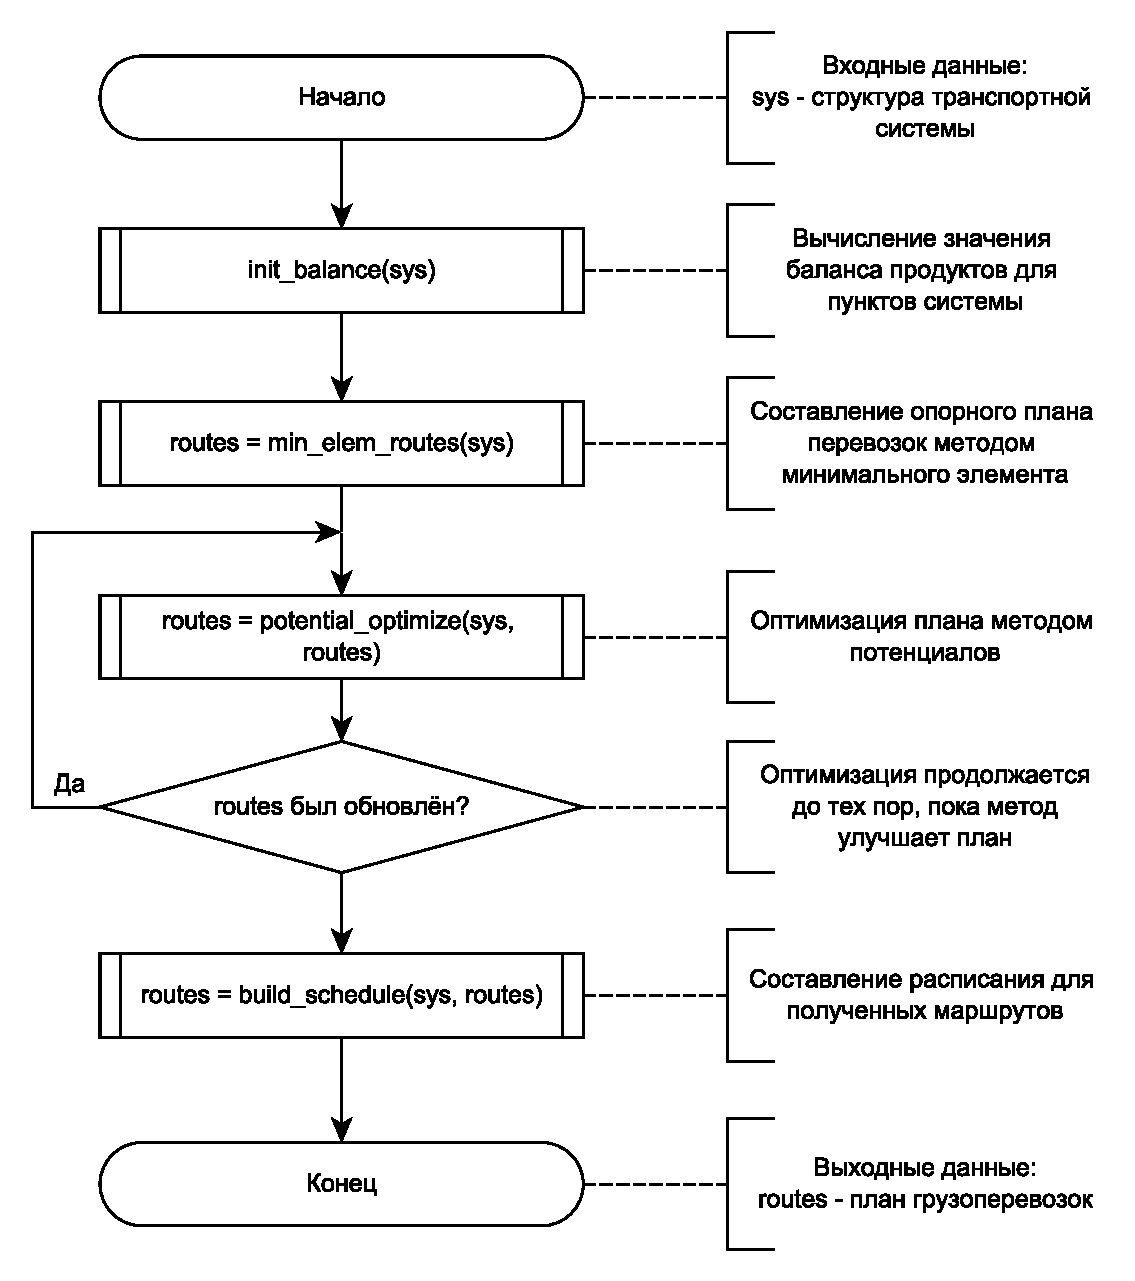
\includegraphics[scale=0.7, angle=0, page=1]{img/algorithms/main.pdf}}
		\caption{Схема общего алгоритма программы}
		\label{alg:main}
	\end{center}
\end{figure}

\textbf{Вычисление начального баланса}

При выполнения алгоритма вычислении баланса, схема которого изображена на рисунке \ref{alg:balance}, для всех складов значение выставляется как количество хранимой продукции, для всех потребителей число заказанных тар продуктов со знаком минус. Баланс стоянки нулевой. Данный этап нужен для проверки соблюдения ограничения количества продукции в различных пунктах. 

\pagebreak
\begin{figure}[h]
	\begin{center}
		{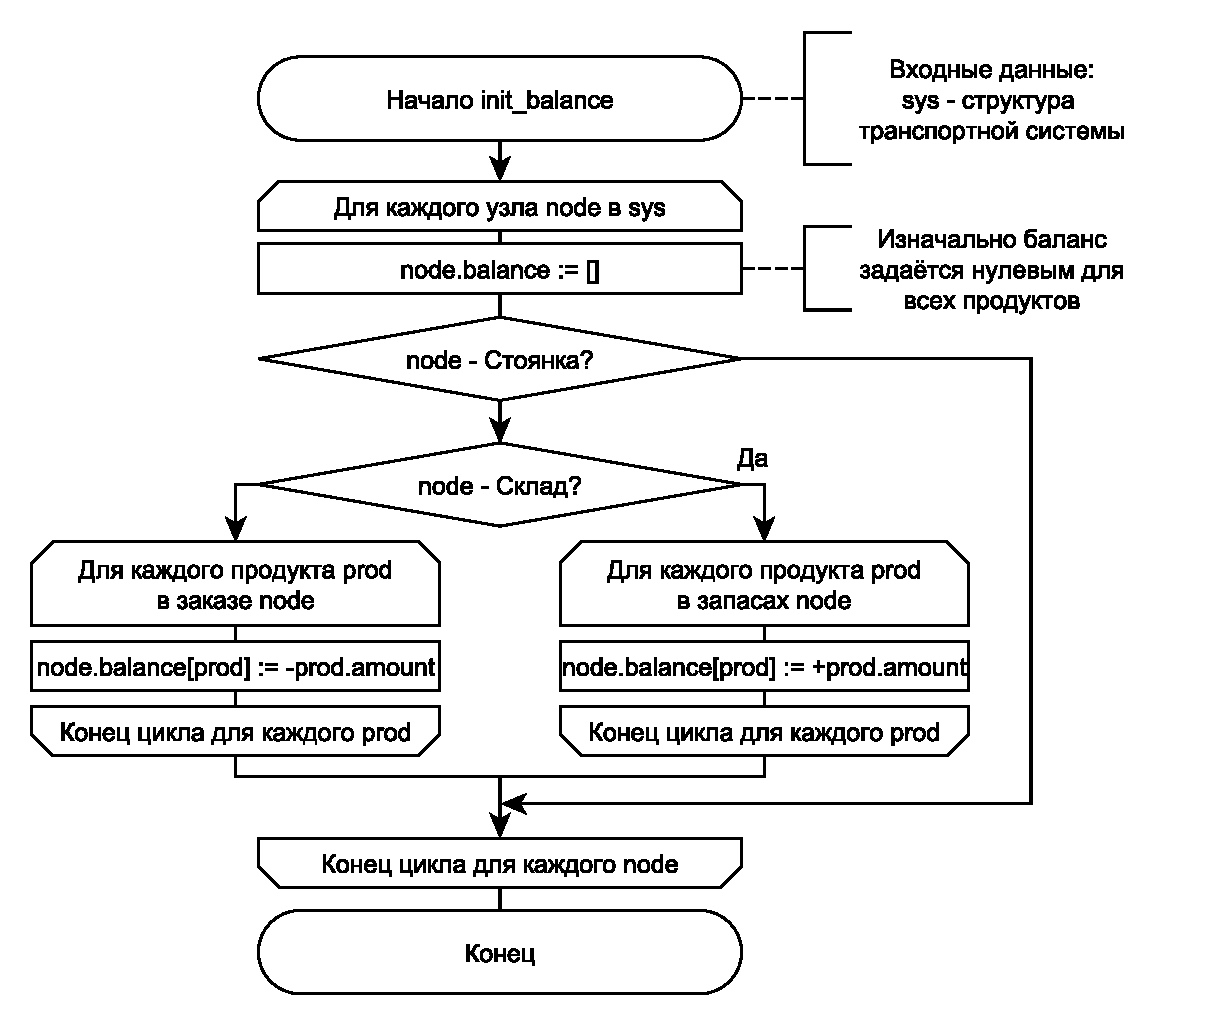
\includegraphics[scale=0.7, angle=0, page=1]{img/init_balance.pdf}}
		\caption{Схема алгоритма вычисления начального баланса}
		\label{alg:balance}
	\end{center}
\end{figure}

\textbf{Составление опорного плана}

На этом этапе формируется опорный план грузоперевозки. Для этого все маршруты, ведущие к каждому потребителю через склад по вычисленному \, кратчайшему пути, просматриваются в соответствии с методом минимального элемента --- в порядке возрастания их стоимости. Схема данного алгоритма приведена на рисунке \ref{alg:min_elem}.

\begin{figure}[hp]
	\begin{center}
		{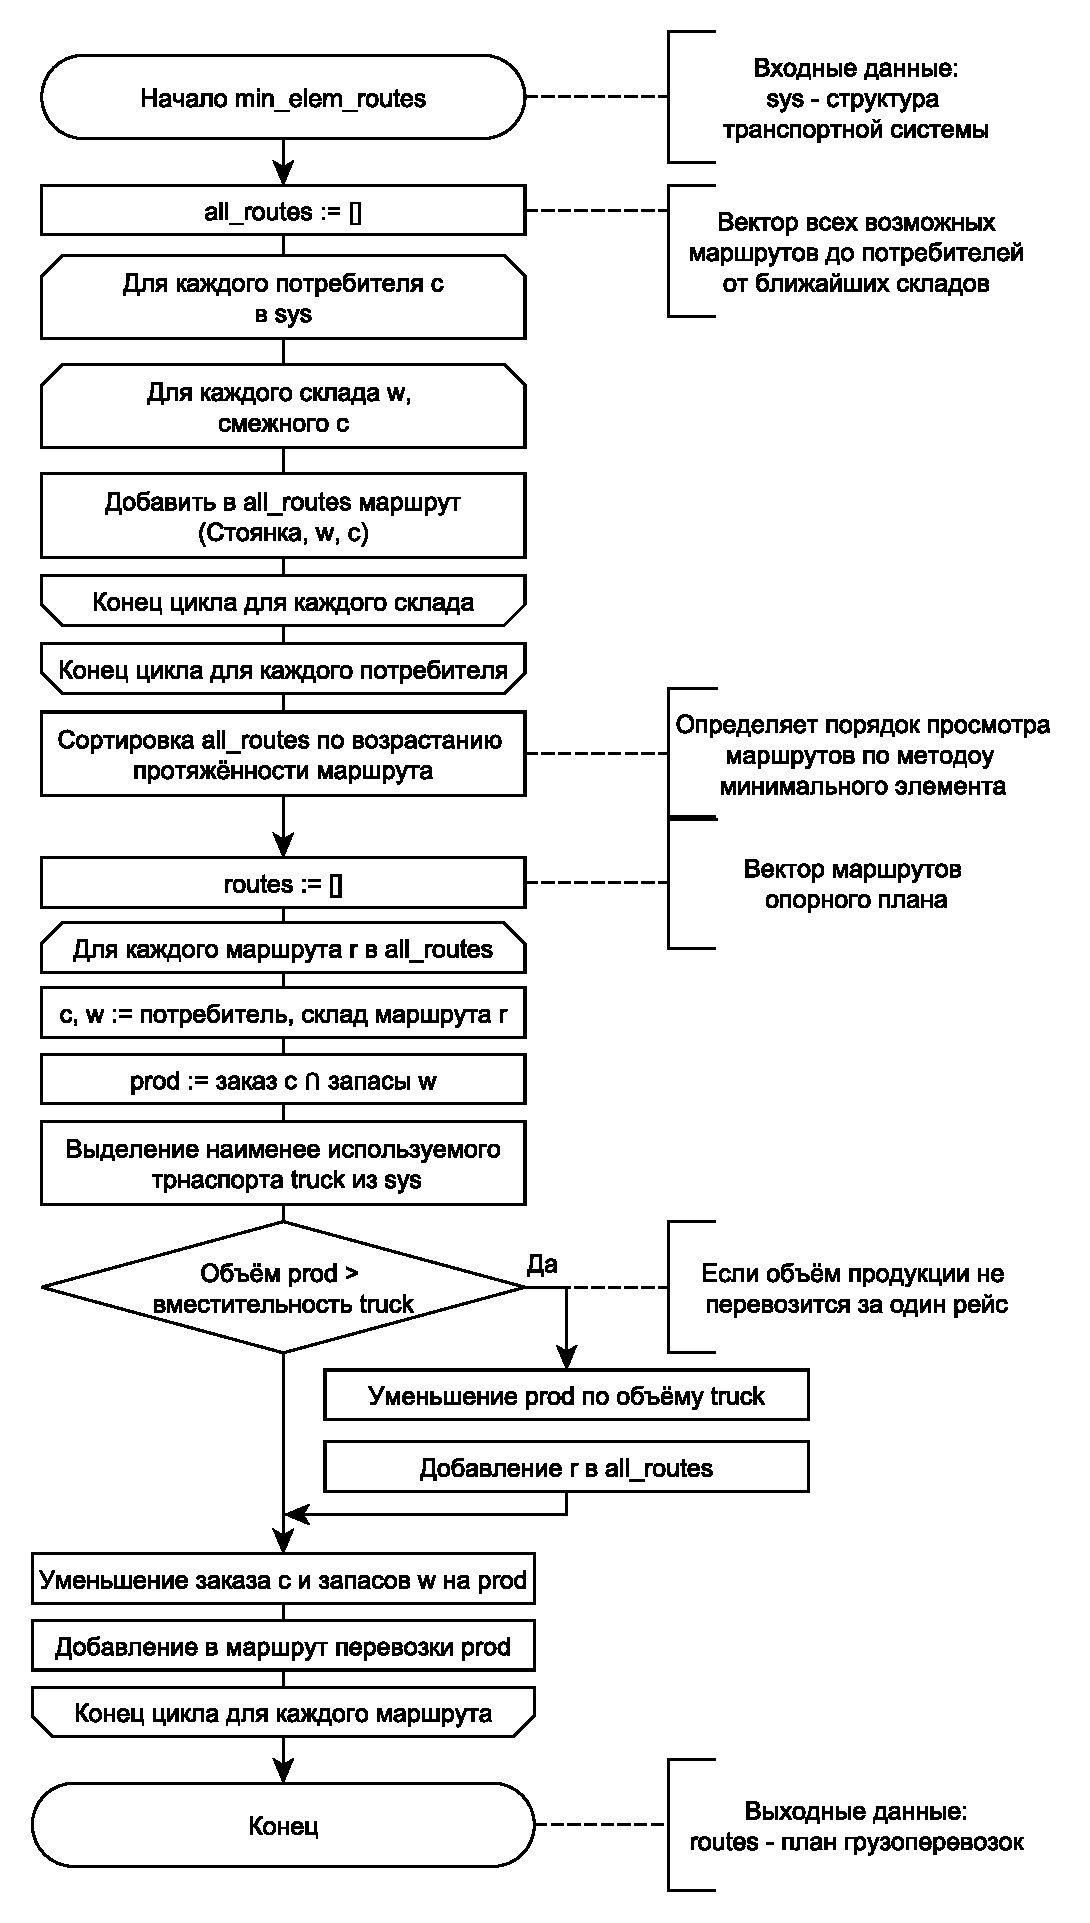
\includegraphics[scale=0.75, angle=0, page=1]{img/min_elem_routes.pdf}}
		\caption{Схема алгоритма минимального элемента}
		\label{alg:min_elem}
	\end{center}
\end{figure}

\textbf{Оптимизация плана}

Рисунки \ref{alg:potential_1} - \ref{alg:potential_2} описывают алгоритм оптимизации плана. После вычисления потенциалов начинается рассмотрение узлов, для которых обнаружены отрицательные невязки. Анализируется возможность замены перевозки текущих маршрутов альтернативными, завершающимися на смежных пунктах. Другие маршруты продлеваются по очереди убывания их выгодности для данного пункта и по мере ограничений.

Если после замены оригинального маршрута в данном пункте функция стоимости для плана становится меньше, то изменения принимаются за новый опорный план. Иначе, поиск путей оптимизации продолжается далее.

\begin{figure}[h]
	\begin{center}
		{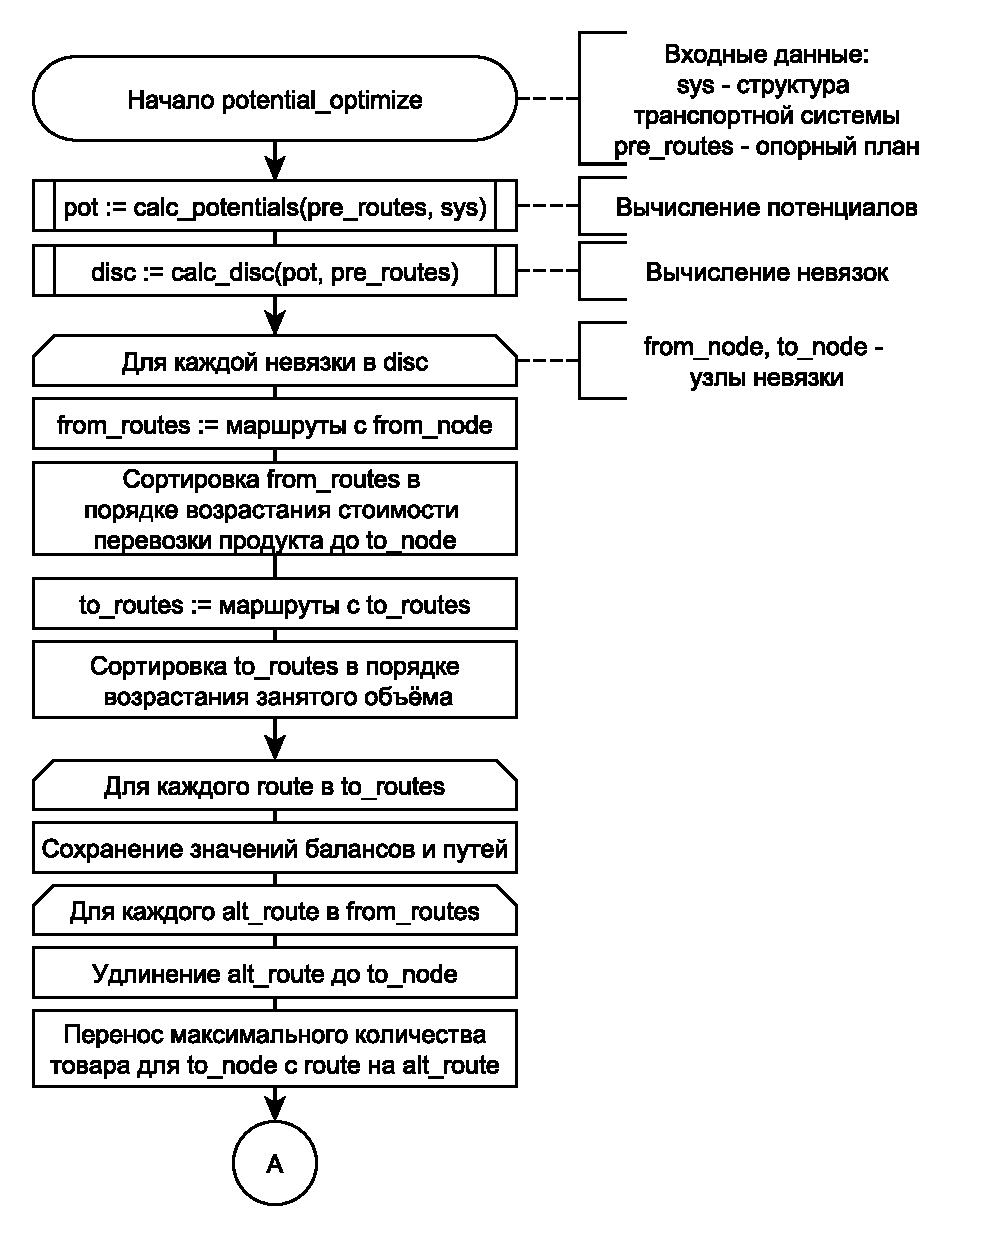
\includegraphics[scale=0.8, angle=0, page=1]{img/potential_optimize_1.pdf}}
		\caption{Схема алгоритма оптимизации}
		\label{alg:potential_1}
	\end{center}
\end{figure}

\begin{figure}[h]
	\begin{center}
		{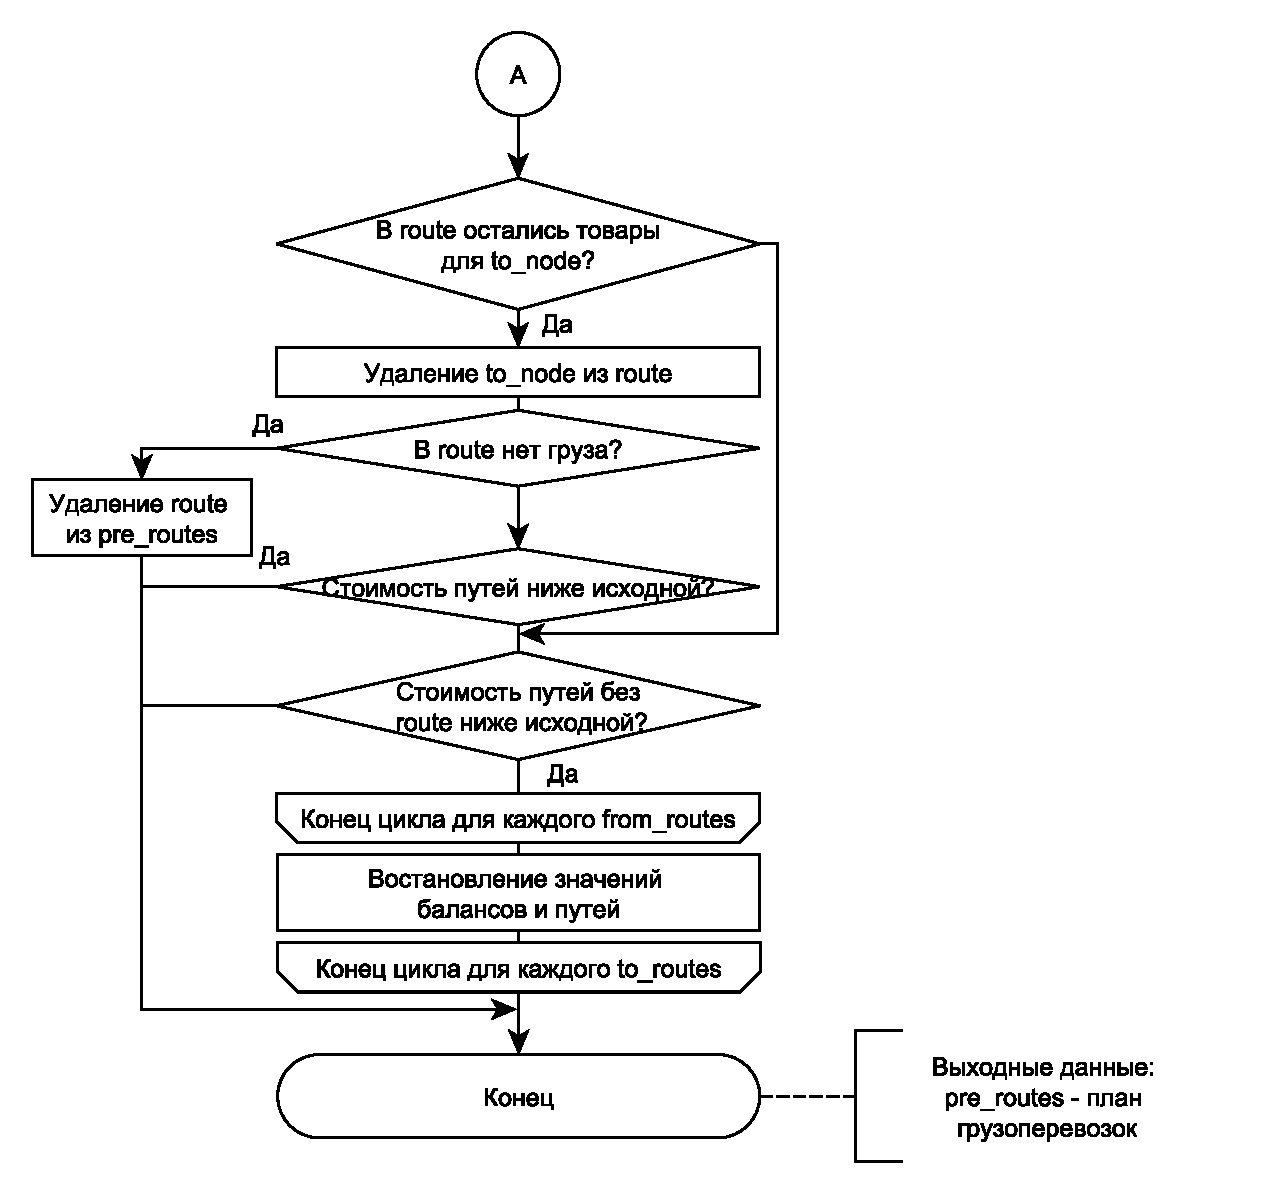
\includegraphics[scale=0.7, angle=0, page=1]{img/potential_optimize_2.pdf}}
		\caption{Схема алгоритма оптимизации (продолжение)}
		\label{alg:potential_2}
	\end{center}
\end{figure}

\pagebreak
\textbf{Формирование расписания}

Рисунок \ref{alg:schedule} описывает алгоритм формирования расписания. Изначально все маршруты выставляются на начало рабочего дня, формируется время прибытия и отбытия из каждого пункта маршрута.

Далее осуществляется поочерёдное рассмотрение расписаний маршрутов, если оно не пересекается с уже принятыми, то маршрут добавляется в общее расписании с закреплением транспорта. Пересечением называется остановка на одном пункте в одинаковый промежуток времени. Величиной пересечения является общее время нахождения на пункте.

\begin{figure}[hp]
	\begin{center}
		{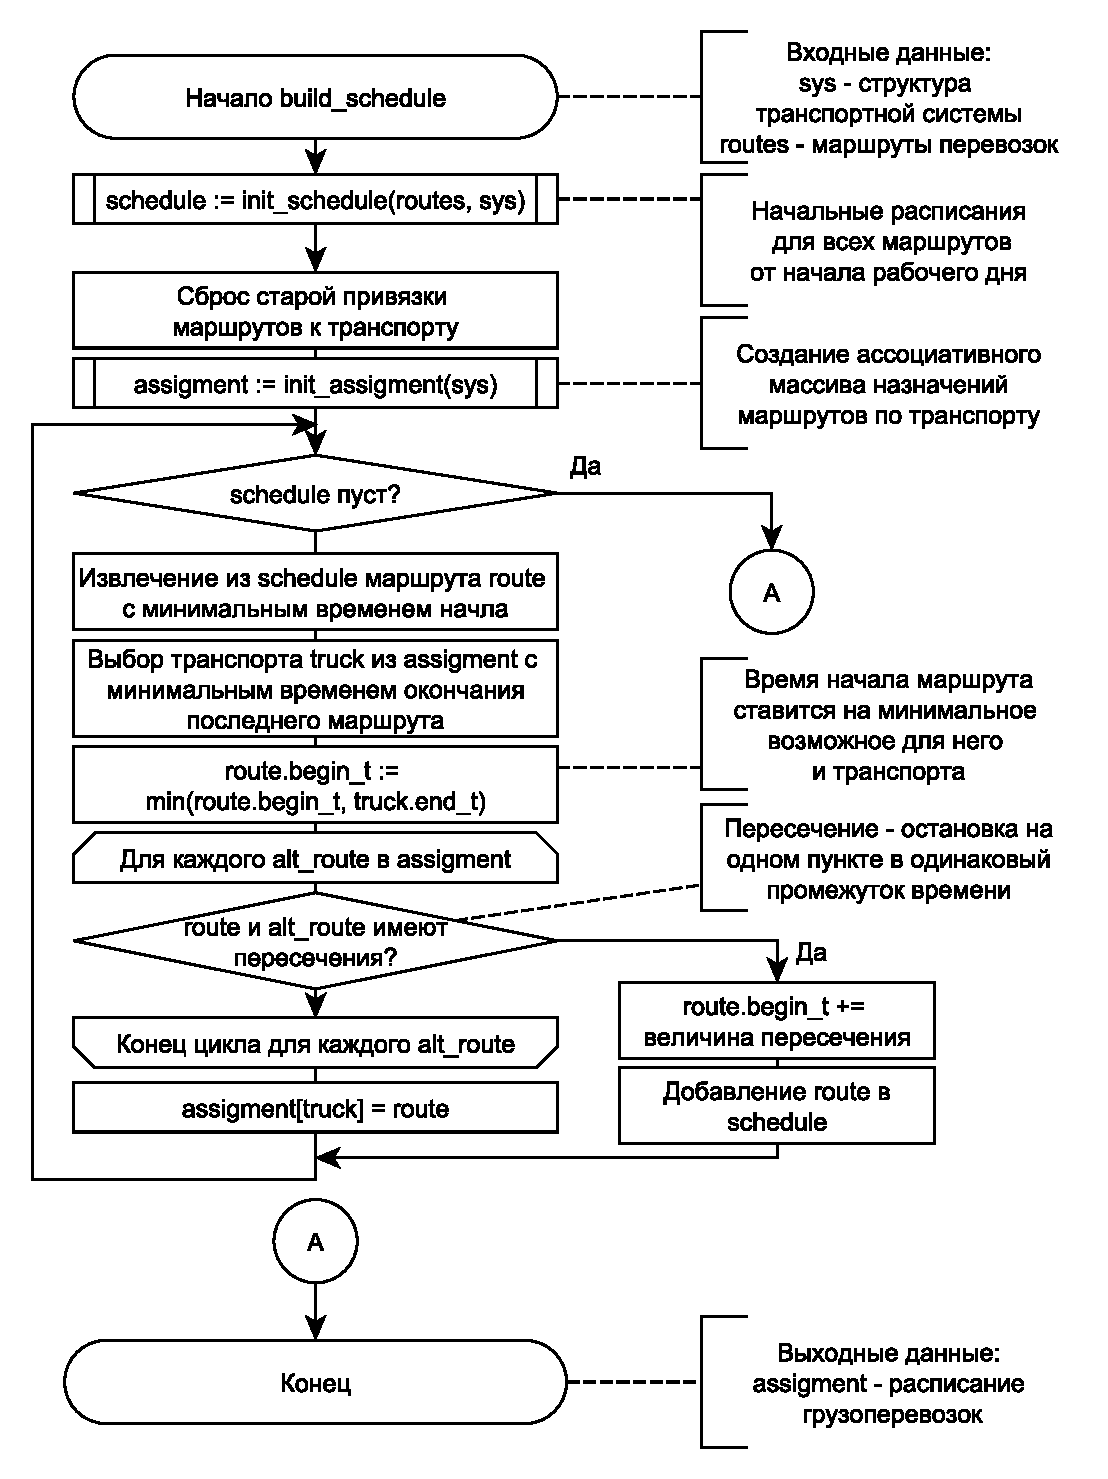
\includegraphics[scale=0.95, angle=0, page=1]{img/schedule.pdf}}
		\caption{Схема алгоритма составления расписания}
		\label{alg:schedule}
	\end{center}
\end{figure}

\subsection{Схема сущностей транспортной системы}
В соответствии с ранее описанной математической моделью, в системе должны быть представлены сущности, \, изображённые на рисунке \ref{ER} c использованием ER-диаграммы.

Ключевым элементом является структура транспортной системы, содержащей в себе все пункты маршрутов. Рёбра транспортного графа описываются с помошью сущности дороги, связывающей два пункта маршрута.
\begin{figure}[h]
	\begin{center}
		{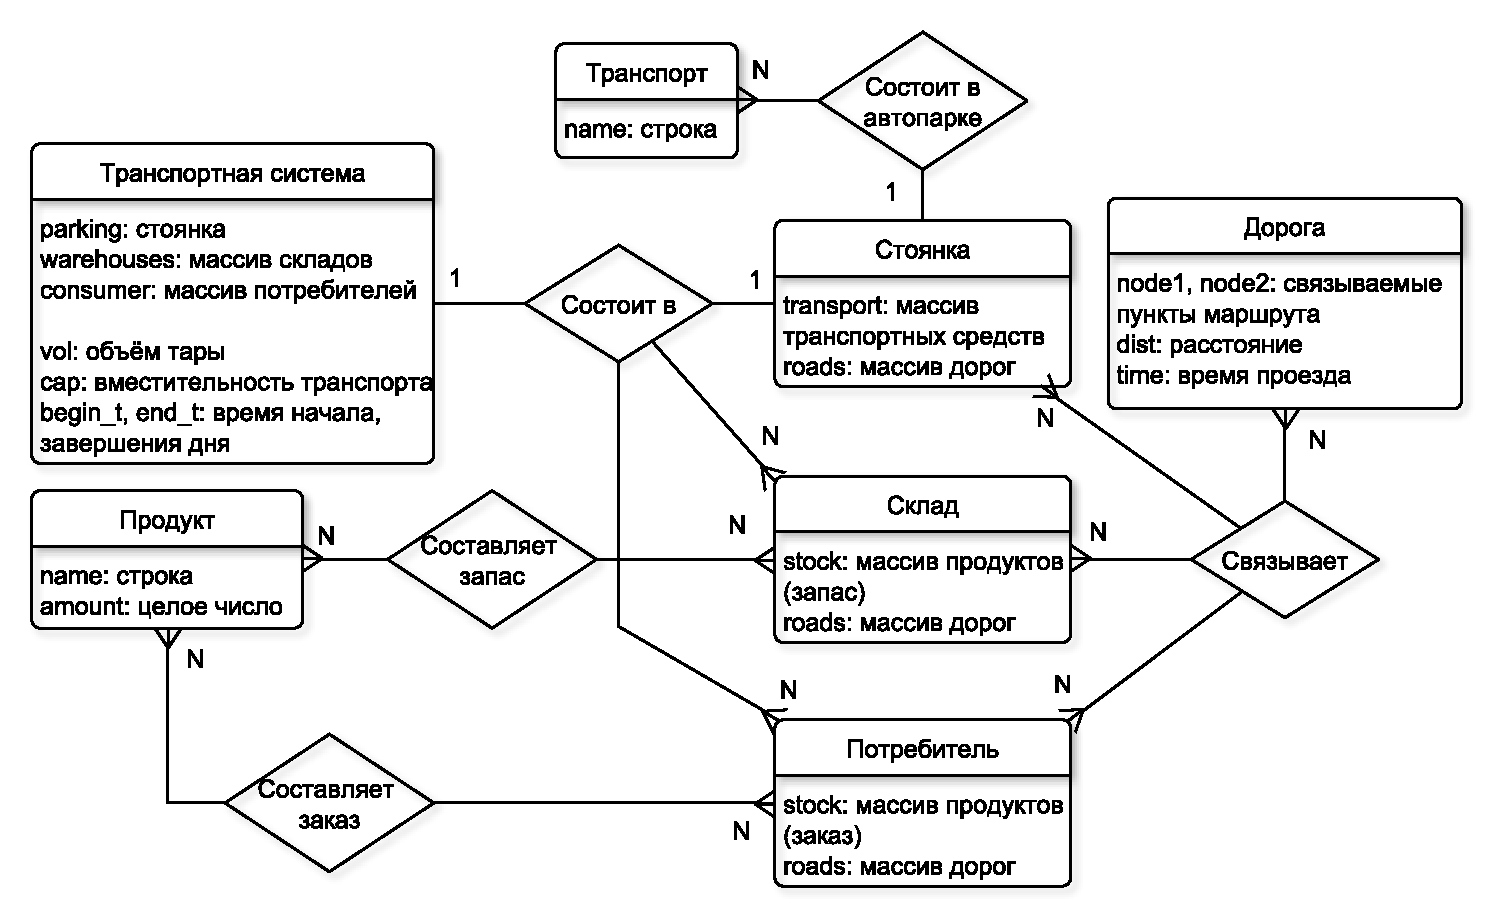
\includegraphics[scale=0.65, angle=0, page=1]{img/ER.pdf}}
		\caption{ER-диаграмма сущностей транспортной системы}
		\label{ER}
	\end{center}
\end{figure}

\subsection{Формат входных данных}
В качестве входных данных выступает описание транспортной системы. Оно должно содержать в себе следующую информацию:

\begin{itemize}
	\item Список всех пунктов маршрута.
	\item Вместительность (в м$^3$) и количество транспорта.
	\item Список запасов складов. Каждый склад описывается списком продуктов (название и количество тар).
	\item Список заказов потребителей -- аналогично запасам складов.
	\item Список дорог: два связанных пункта, расстояние (в км.), время проезда (в мин.).
	\item Объём одной тары в (в м$^3$).
	\item Время начала и завершения рабочего дня.
\end{itemize}

\subsection{Формат выходных данных}
В качестве выходных данных выступает описание плана грузоперевозок. Оно состоит из списка маршрутов, каждый из которых должен содержать в себе следующую информацию:

\begin{itemize}
	\item Последовательность посещения пунктов.
	\item Номер привязанного транспортного средства.
	\item Список товаров, загружаемых или выгружаемых на каждом пункте.
	\item Список времени прибытия и отбытия в каждый пункт маршрута.
\end{itemize}	

\subsection*{Вывод}
В данном разделе были представленны IDEF0 и ER диаграммы, схемы алгоритмов. Описан формат входных и выходных данных программы.

\pagebreak